% !TeX spellcheck = en_US
\documentclass[french]{yLectureNote}

\title{Mécanique}
\subtitle{Mécanique du point}
\author{Paulhenry Saux}
\date{\today}
\yLanguage{Français}

\professor{S.Deheuvels}%sebastien.deveuhels.irap.omp.eu

\usepackage{graphicx}%----pour mettre des images
\usepackage[utf8]{inputenc}%---encodage
\usepackage{geometry}%---pour modifier les tailles et mettre a4paper
%\usepackage{awesomebox}%---pour les boites d'exercices, de pbq et de croquis ---d\'esactiv\'e pour les TP de PC
\usepackage{tikz}%---pour deiffner + d\'ependance de chemfig
\usepackage{tkz-tab}
\usepackage{chemfig}%---pour deiffner formules chimiques
\usepackage{chemformula}%---pour les formules chimiques en \'equation : \ch{...}
\usepackage{tabularx}%---pour dimensionner automatiquement les tableaux avec variable X
\usepackage{awesomebox}%---Pour les boites info, danger et autres
\usepackage{menukeys}%---Pour deiffner les touches de Calculatrice
\usepackage{fancyhdr}%---pour les en-t\^ete personnalis\'ees
\usepackage{blindtext}%---pour les liens
\usepackage{hyperref}%---pour les liens (\`a mettre en dernier)
\usepackage{caption}%---pour la francisation de la l\'egende table vers Tableau
\usepackage{pifont}
\usepackage{array}%---pour les tableaux
\usepackage{lipsum}
\usepackage{makecell}
\usepackage{yFlatTable}
\usepackage{multicol}
\newcommand{\Lim}[1]{\lim\limits_{\substack{#1}}\:}
\renewcommand{\vec}{\overrightarrow}
\newcommand{\norm}[1]{||\vec{#1}||}
\DeclareMathOperator\arctanh{arctanh}
\begin{document}

%\titleOne
\setcounter{chapter}{5}
	\chapter{Oscillateurs}
	\section{Ressort}

\subsection{Ressort}
\begin{theorem}[Force de rappel d'un ressort]
\[ - \vec{F_r} = k(x-l_0)\vec{e_x}\] avec $l_0$ la longueur à vide et $k$ la constante de raideur
\end{theorem}

Souvent, on prend pour origine du repère la longueur à vide du ressort. Dans ce cas, l'allongement du ressort vaut $x$.

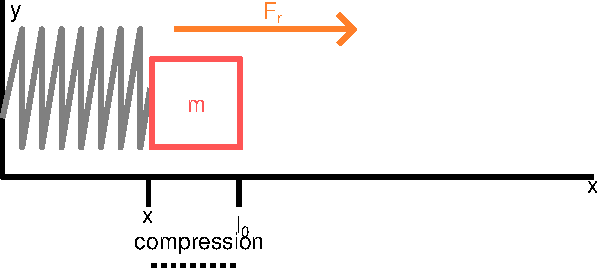
\includegraphics[scale=0.5]{compression}\: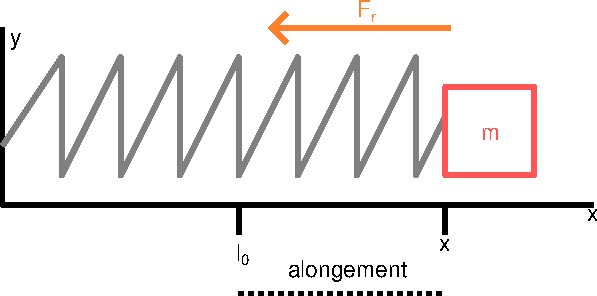
\includegraphics[scale=0.5]{alongement}

\section{Oscillateur harmonique (OH)}
On appelle \emph{ocillateur harmonique} un système qui répond à l'EQD suivante :
\[\frac{\mathrm{d}^2x}{\mathrm{d}t^2}+ \omega_0^2x(t) = 0\]

Elle est du second ordre linéaire à coefficient constant sans terme du premier ordre.\marginInfo{Conditions nécéssaires : Si le coefficient du terme du second ordre est égal à 1, le coefficient du terme d'ordre 0 est positif}

Exemple : $\ddot{x}+4x = 0$ est un OH mais pas $\ddot{x}-x=0$
\subsection{Résolution}
On cherche des solutions de la forme
\begin{flalign}
x&= Ce^{rt}\label{solution_generale}\\
\dot{x} &= Cre^{rt}\notag\\
\ddot{x} &= Cr^2e^{rt}\notag
\end{flalign}
On injecte \eqref{solution_generale} dans l'EQD pour obtenir l'équation caractéristique
\begin{flalign*}
r^2+\omega_0^2 &= 0\\
\iff r^2 &= -\omega_0^2\\
\iff r &= \pm i\omega_0
\end{flalign*}

La solution est complexe et peut s'écrire sous 3 formes :
\begin{theorem}[Solutions d'un OH]
\begin{itemize}
 \item $x(t) = \underline{C_1}e^{-i\omega_0t} + \underline{C_2}e^{+i\omega_0t}$
\item $x(t) = A\cos(\omega_0t) + B\sin(\omega_0t)$
\item $x(t) = C\cos(\omega_0t+\varphi) \text{ou }x(t) = D\sin(\omega_0t+\eta$
\end{itemize}
\end{theorem}
Chacune des solutions fait intervenir 2 constantes d'intégration que l'on détermine en appliquant les conditions initiales sur $x(t)$ et $\dot{x}(t)$.

\checkInfo{Exemple du ressort}{
La solution de l'EQD est $x(t) = A\cos(\omega_0t) + B\sin(\omega_0t)$

Si à $t=0$, on allonge le ressort sur uns distance $x(0) = x_m$ et on étudie le mouvement sans vitesse initiale ($\dot{x}(0) = 0$).

$x(0) = x_m = A\times 1$.

Il faut calculer $\dot{x}(t) = - A\omega_0\sin(\omega_0t) + B\omega_0\sin(\omega_0t)$, donc $\dot{x}(0) = B\omega_0 = 0$ car pas de vitesse initiale, donc $B=0$

On obtient alors $x(t) = x_m\cos(\omega_0t)$ et $\dot{x} = -x_m \omega_0 \sin(\omega_0t)$.}

\subsubsection{Période T des oscillations}
\begin{theorem}[Période]
\[T = \frac{2\pi}{\omega_0}\]
\end{theorem}

\subsubsection{Représentation graphique}
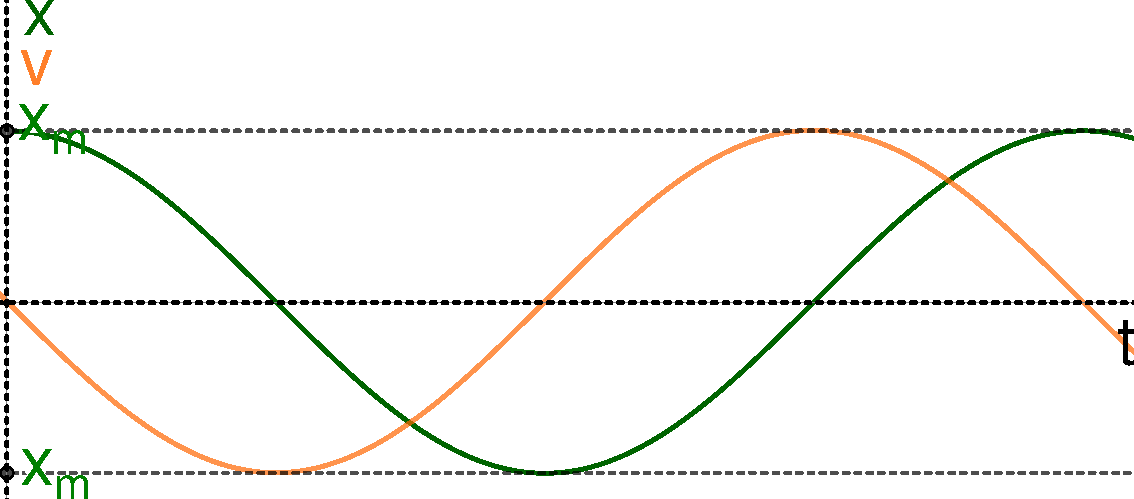
\includegraphics[scale=0.4]{representation_1}

Quand l'amplitude des oscillations est maximale, la vitesse est nulle et quand $x$ est nul, la vitesse est maximale.\marginInfo{Vitesse et position sont dits en quadrature de phase.}
\section{Oscillateurs amortis}
\subsection{En résumé (par coeur)}
	\begin{tabular}{_c^c^c^c^c}
		\tableHeaderStyle%
		Régime & $\Delta$ & $Q = \omega_0\tau$ & Représentation & Solution\\
		Pseudo-périodique & $<0$ & $>1/2$& 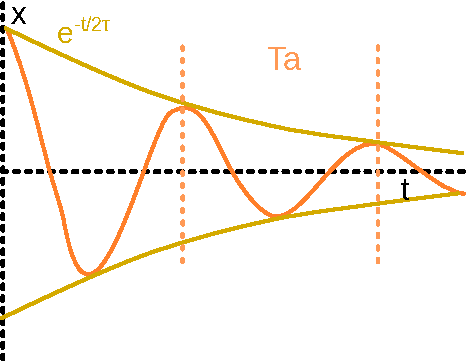
\includegraphics[scale=0.2]{pesudo} & \makecell{$x(t) = e^{-\frac{t}{2\tau}} (A\cos(\omega_at) + B\sin(\omega_at))$ avec $\omega_a = \omega_0\sqrt{1-\frac{1}{4Q^2}}$}\\
		Critique & $=0$ & $=1/2$ & 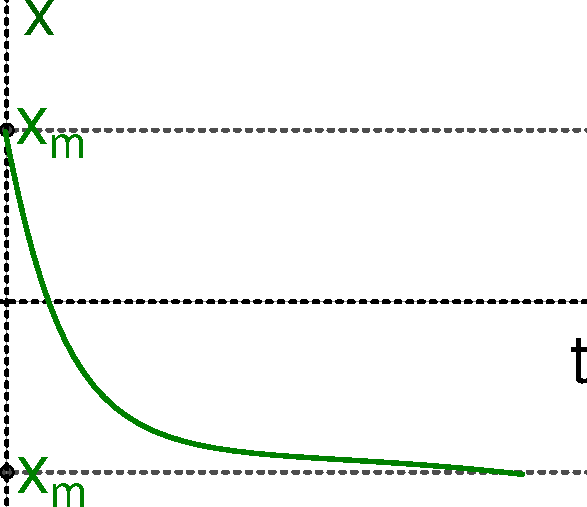
\includegraphics[scale=0.2]{delta0} & $x(t) = (C_1+C_2t)e^{-\frac{1}{2\tau}t}$\\
		Apériodique & $>0$ & $<1/2$ &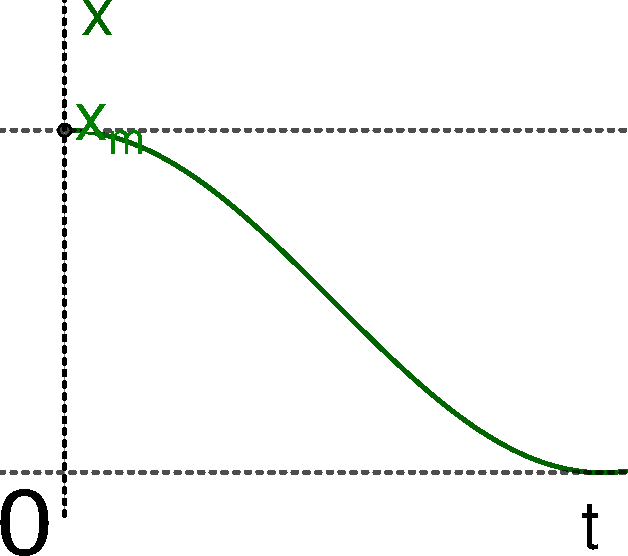
\includegraphics[scale=0.2]{aper} & \makecell{$x(t) = e^{-\frac{t}{2\tau}}(C_1e^{-\beta t} + C_2e^{+\beta t})$ \\avec $\beta = \omega_0\sqrt{-1+\frac{1}{4Q^2}}$}
	\end{tabular}
\subsection{Mise en équation}
On revient au cas du ressort étiré et on considère en plus une force de frottement fluide $\vec{F_f} = -\alpha \vec{v}$. On a toujours, à $t=0$, $x(0) = x_m$ et $\dot{x}(0) = 0$

Bilan des forces : $\vec{P},\vec{R},\vec{F_r},\vec{F_f}$.

On applique le PFD : $m\vec{a} = \vec{P}+\vec{R}+\vec{F_r}+\vec{F_f}$
\[\left\{\begin{matrix}
 m\ddot{x} &= 0 + 0 -kx -\alpha \dot{x}\\
 m\ddot{y} &= -mg+R + 0 -\alpha\dot{y}
\end{matrix}\right.\]

Pas de mouvement selon $y$, donc $y=\dot{y} = \ddot{y} = 0$
\begin{equation}\left\{\begin{matrix}
 m\ddot{x} &=-kx -\alpha \dot{x}\\
0 &= -mg+R + 0 \Rightarrow R = mg
\end{matrix}\right.\label{systeme_1}\end{equation}

On remarque que les forces de frottement ajoutent un terme du premier ordre. On obtient de \eqref{systeme_1} l'EQD
\begin{equation}\ddot{x} + \frac{\alpha}{m}\dot{x} + \frac{k}{m}x = 0\label{eqd_1}\end{equation}

On peut écrire \eqref{eqd_1} sous forme canonique, avec $\tau = \frac{m}{\alpha}$ et $\omega_0 = \sqrt{\frac{k}{m}}$ :
\begin{equation}\ddot{x} + \frac{1}{\tau}\dot{x} + \omega_0^2x = 0\label{eqd_1_h}\end{equation}

\subsection{Résolution}
\eqref{eqd_1_h} est homogène, on cherche des solutions sous la forme $Ce^{rt}$

L'équation caractéristique de \eqref{eqd_1_h} est : \begin{equation}r^2 + \frac{1}{\tau}r + \omega_0^2 = 0\label{eq_c_1}\end{equation}

\eqref{eq_c_1} est du second degré dont on calcule le discriminant ! \begin{equation}\Delta = \frac{1}{\tau^2} - 4\omega_0^2 = \frac{1}{\tau^2}(1-4\omega_0^2\tau^2)\label{delta}\end{equation} Cela fait intervenir la grandeur $Q = \omega_0\tau$ appelé \emph{facteur de qualité}, sans dimensions.
\subsubsection{Temps}
$\omega_0 = \frac{2\pi}{T}$ avec $T$ la période de l'OH, en l'absence de frottement

$\tau$ est le temps caractéristique sur lequel les frottements opèrent.

$Q = \omega_0\tau = 2\pi\frac{\tau}{T}$

Si $Q>> 1$, les frottements n'ont pas le temps d'agir pendant une période d'oscillation : on se rapproche de l'OH, car $\tau >> T$

Si $Q<<1 \iff \tau << T$, on s'attend à ce que les frottements emp\^echent les oscillations.

\end{document}

